\chapter{Evaluation und Validation}
\label{ch:Eval}

Die  Softwarearchitektur wurde während der Realisierung mit einem kleineren Datensatz mit 100000 Ratings getestet. Nach Beendigung der Realisierung der Softwarearchitektur, wurde festgestellt, das mit den gegebenen Ressourcen, keine Berechnung der Top $N$ Nachbarn mit 25 Millionen Ratings möglich ist.
Nach Absprache mit dem Betreuer Tahir Majeed, wurden die Top N Nachbarn mit 1 Million, 2 Millionen, 5 Millionen und 7 Millionen Ratings berechnet. 

\begin{figure}[htb]
	\centering
	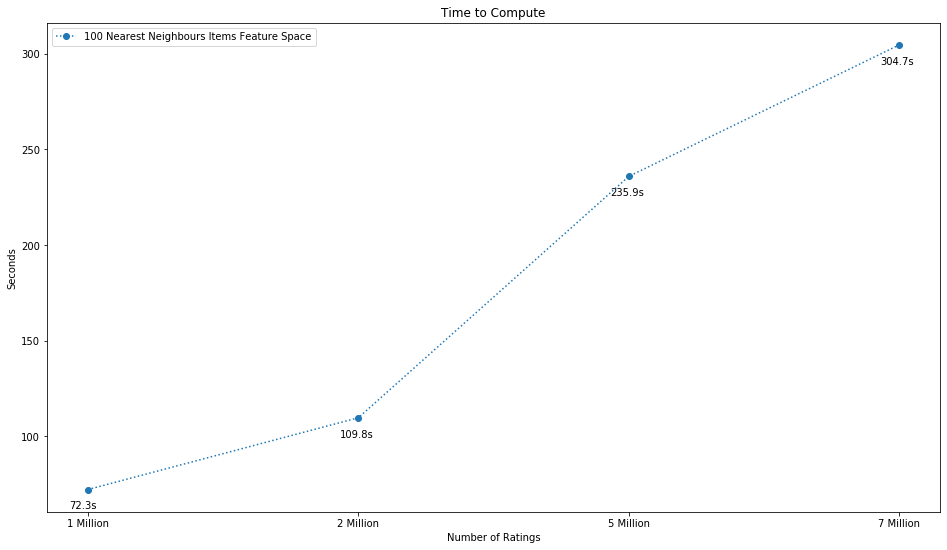
\includegraphics[keepaspectratio,width=\linewidth]{img/Time to Compute Items Featurespace.png}
	\caption{Rechenzeit Top 100 Item Nachbarn Featurespace}
	\label{fig:Rechenzeit Itemnachbarn Featurespace}
\end{figure}

In Abbildung \ref{fig:Rechenzeit Itemnachbarn Featurespace} sieht man, dass die Rechenzeit von 304 Sekunden (ungefähr 5 Minuten) im Featurespace auch mit 7 Millionen Ratings relativ kurz ist. Auch die Berechnung der Top 100 User Nachbaren ist mit 596 Sekunden (ungefähr 10 Minuten), wie in Abbildung \ref{fig:Rechenzeit Usernachbarn Featurespace} ersichtlich, relativ schnell. 

\begin{figure}[h!tb]
	\centering
	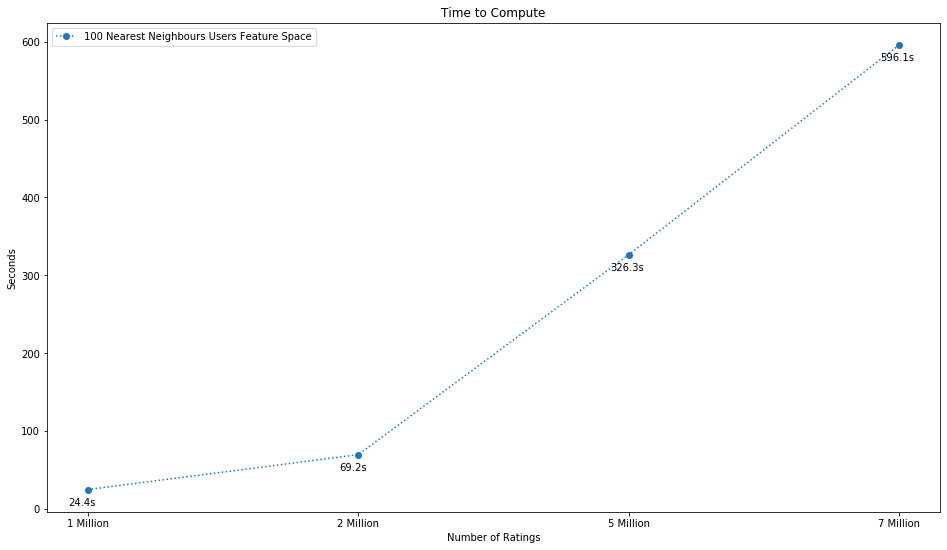
\includegraphics[keepaspectratio,width=\linewidth]{img/Time to Compute User Featurespace.png} 
	\caption{Rechenzeit Top 100 User Nachbarn Featurespace}
	\label{fig:Rechenzeit Usernachbarn Featurespace}
\end{figure}
Wie in Abbildung \ref{fig:Rechenzeit Featurespace} zu sehen ist, sieht man aber schon einen Unterschied zwischen der Berechnung der User und Item Nachbarn.
\begin{figure}[h!tb]
	\centering
	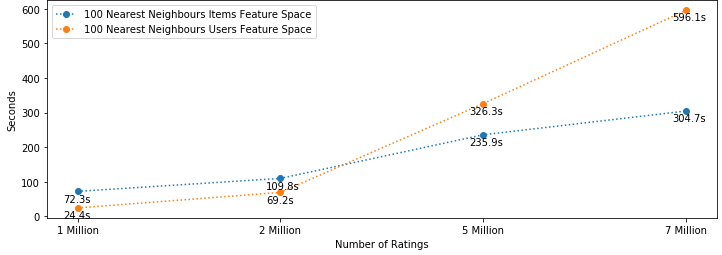
\includegraphics[keepaspectratio,width=\linewidth]{img/Time to Compute Featurespace.png} 
	\caption{Rechenzeit Top 100 Nachbarn Featurespace}
	\label{fig:Rechenzeit Featurespace}
\end{figure}

%TODO Einfügen von Abbildung und Referenz
Werden aber die Top 100 Nachbarn im PCA Space gesucht explodiert die Rechenzeit enorm. Wieder mit 1 Million Ratings beginnend, starten wir bei der Berechnung der 100 Top Item Nachbarn im PCA Space bei einer Rechenzeit von 675 Sekunden (siehe Abbildung \ref{fig:Rechenzeit Items PCA} ). Dies überschreitet bereits mit nur 1 Million Ratings die Rechenzeit der Top 100 Item und User Nachbarn im Featurespace. Betrachten wir nun die Rechenzeit für 2 Millionen Ratings aus Abbildung \ref{fig:Rechenzeit Items PCA}, sehen wir, dass die Rechenzeit mit 4112 Sekunden (circa 69 Minuten) bereits jetzt um das \textbf{sechsfache} gestiegen ist. Um die Berechnung für 5 Millionen Ratings zu erstellen werden bereits 52107.37 Sekunden (14,47 Stunden) benötigt, was circa das \textbf{Zwölffache} der Berechnungszeit mit 2 Millionen Ratings entspricht. Um die Zeitkomplexität für 7 Millionen Ratings abzuschätzen wird die Berechnungszeit des Datensets mit 5 Millionen Ratings, wieder mit 12 multipliziert. Dies ist sehr minimalistisch geschätzt, betrachtet man die Wachstumskurve sieht man, dass die Zeit exponentiell steigt. Mit Faktor 12 gerechnet, kommt man auf eine Berechnungszeit von 7.2 Tagen für 7 Millionen Ratings.


\begin{figure}[h!tb]
	\centering
	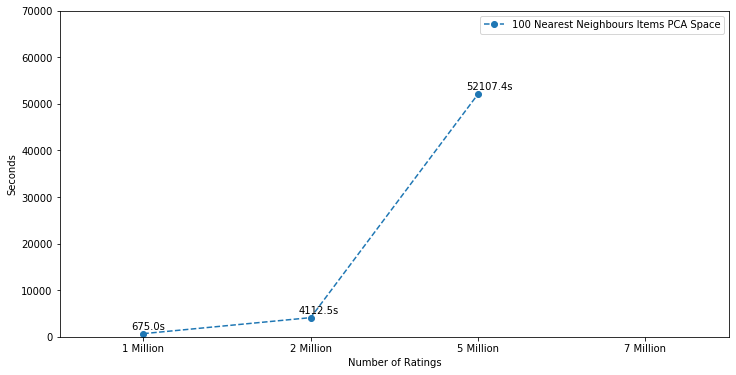
\includegraphics[keepaspectratio,width=\linewidth]{img/Time to Compute Items PCA.png} 
	\caption{Rechenzeit Item Nachbarn PCA Space}
	\label{fig:Rechenzeit Items PCA}
\end{figure}


Sehen wir uns die Kurve der Zeitkomplexität der Berechnung der Top 100 User im PCA Space an (Abbildung \ref{fig:Rechenzeit User PCA}, sehen wir einen relativ identischen Verlauf, wie bei der Zeitkomplexität der Top 100 Item Nachbarn im PCA Space. 

\begin{figure}[h!tb]
	\centering
	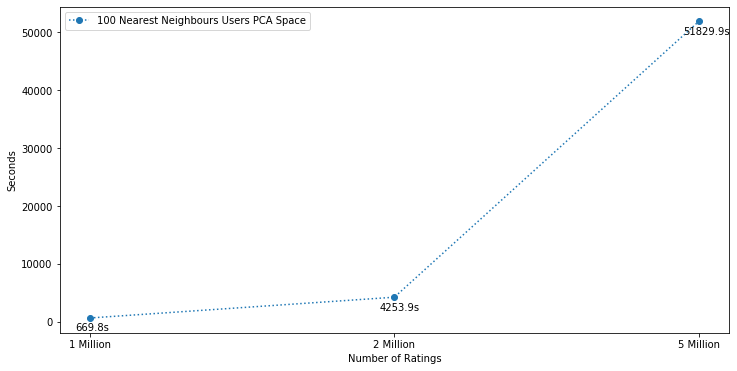
\includegraphics[keepaspectratio,width=\linewidth]{img/Time to Compute User PCA.png} 
	\caption{Rechenzeit User Nachbarn PCA Space}
	\label{fig:Rechenzeit User PCA}
\end{figure}

Dies ist nicht nur den ähnlichen Kurven aus den Abbildungen \ref{fig:Rechenzeit Items PCA} und \ref{fig:Rechenzeit User PCA} zu entnehmen, sondern wird weiter auch durch Abbildung \ref{fig:Rechenzeit PCA} verdeutlicht.

\begin{figure}[h!tb]
	\centering
	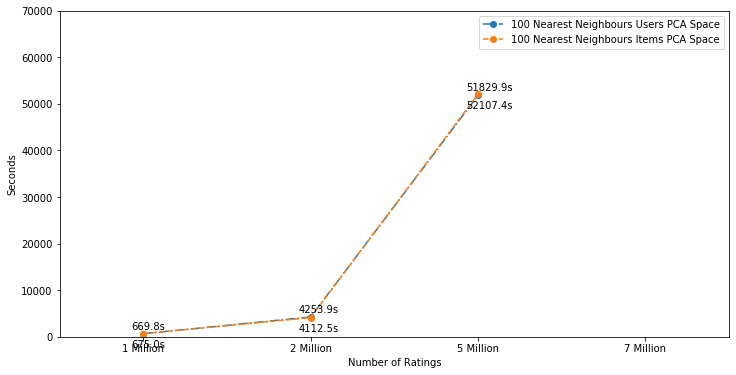
\includegraphics[keepaspectratio,width=\linewidth]{img/Time to Compute PCA.png} 
	\caption{Rechenzeit Top 100 Nachbarn PCA Space}
	\label{fig:Rechenzeit PCA}
\end{figure}

Auf Grund der geschätzen Berechnungszeit für die Top 100 Nachbarn im PCA Space mit 7 Millionen Ratings von ungefähr 7 Tagen für je die Item und User Nachbarn, wurde entschieden diese nicht zu berechnen.

Schauen wir uns alle Kurven der Rechenzeit un Abbildung \ref{fig:Rechenzeit Total}  an, sieht man, dass die Rechenzeit im Feature Space, verglichen mit der Rechenzeit im PCA Space, vernachlässigbar ist.

\begin{figure}[h!tb]
	\centering
	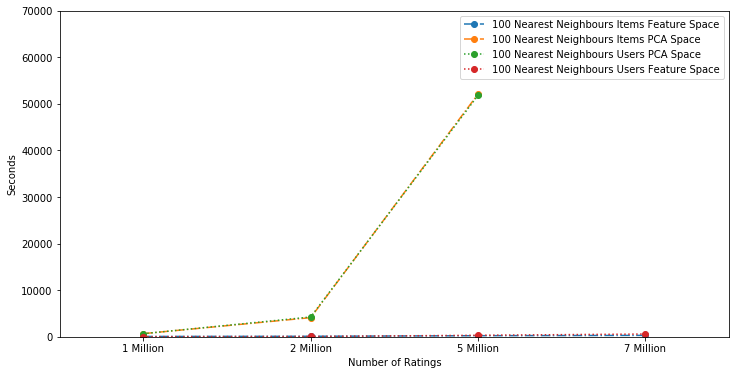
\includegraphics[keepaspectratio,width=\linewidth]{img/Time to Compute all 5MPCA.png} 
	\caption{Rechenzeit Top 100 Nachbarn}
	\label{fig:Rechenzeit Total}
\end{figure}

Noch deutlicher zu sehen ist dass, wenn die geschätzte Rechenzeit von circa 7 Tagen im PCA Space für die Berechnung des Datensets mit 7 Millionen Ratings der Grafik (Abbildung \ref{fig:Rechenzeit Total Estimated}) hinzugefügt wird. 

\begin{figure}[h!tb]
	\centering
	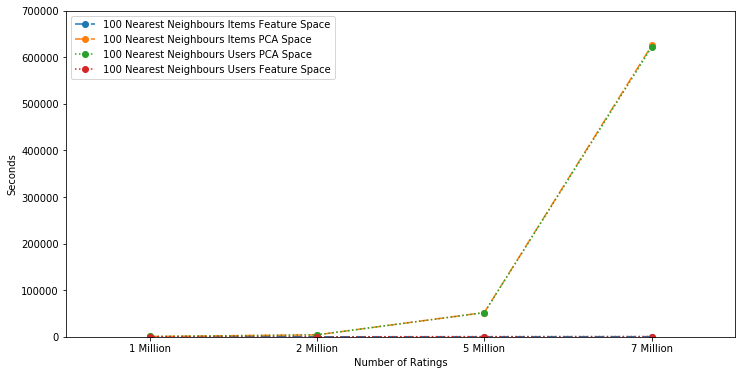
\includegraphics[keepaspectratio,width=\linewidth]{img/Time to Compute all estimated.png} 
	\caption{Rechenzeit Top 100 Nachbarn mit geschätzer Zeit für 7 Millionen Ratings}
	\label{fig:Rechenzeit Total Estimated}
\end{figure}

\section{Resultate}
\subsection{Vergleich der Item Nachbarn mit 1 Million Ratings}
\subsection{Vergleich der Item Nachbarn mit 2 Millionen Ratings}
\subsection{Vergleich der Item Nachbarn mit 5 Millionen Ratings}

\subsection{Vergleich der User Nachbarn mit 1 Million Ratings}
\subsection{Vergleich der User Nachbarn mit 2 Millionen Ratings}
\subsection{Vergleich der User Nachbarn mit 5 Millionen Ratings}


Waren die eingesetzten Methoden zweckmässig?
- Sind die Ergebnisse aussagekräftig und zuverlässig?
- Sind die Ergebnisse auf andere Gebiete übertragbar?
- In welchem Verhältnis stehen die Ergebnisse zur übrigen Forschung? Decken sie sich oder
widersprechen sie ihr?
- Welche Bedeutung haben die Ergebnisse für die Praxis?
- Welche Bedeutung haben die Ergebnisse für weitere Forschungen?

\section{Vergleich mit Anforderungen}
\label{sec:VergleichAnforderungen}
% TODO Vergleich mit Anforderungen Soll<->Ist
Die Produktrandbedingungen aus Kapitel \ref{sec:Produktrandbedingungen} konnten durchgängig erfüllt werden. Die Produktrandbedingung 2 konnte wie zu Beginn des Kapitel \ref{ch:Eval} beschrieben nur teilweise erfüllt werden. Es wurde zwar das Movies 25M Dataset verwendet, jedoch konnten die Berechnungen nicht auf dem gesamten Datenset ausgeführt werden.

Die im Kapitel \ref{sec:Out of Scope} Out of Scope definierte Anforderung wurde wie in Kapitel \ref{ch:Realisierung} besprochen trotzdem umgesetzt.

\section{Technische Aspekte}
% TODO Evaluation der verwendeten Hilfsmittel

\section{Vorgehen}
% TODO Evaluation der verwendeten Arbeitsprozesse
